\documentclass{amsart}
\usepackage{graphicx}
\newcommand*\oct{\vcenter{\hbox{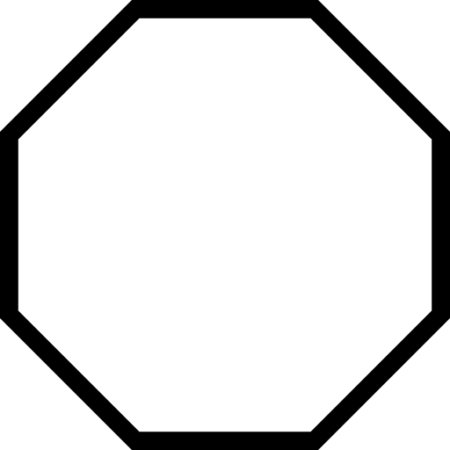
\includegraphics[width=.9em]{octagon.png}}}}
\newcommand{\F}{\mathcal{F}}
\newcommand{\Z}{\mathbb{Z}}
\title{Stopping Times}
\author{Robert Dougherty-Bliss and Charles Kenney}
\begin{document}
\maketitle
Let $$V = \bigoplus_{k=1}^\infty (\Z/2\Z)$$
and
$$\oct_1 = \{0\} \subset V,$$
while for $k \geq 1,$
$$\oct_{2k} = \{v \in V : \forall j > k, v_j = 0, \text{ and } v \text{ has stopping time } 2k \}. $$
Let $g(n) = |\oct_n|.$ Then
$$g(4n) = 2g(4n-2)$$
and
$$g(4n+2) = 2g(4n)-g(2n).$$
Define $e_0, e_1 : V \to V$ by
$$e_0(b) = \begin{cases} 0 \text{ if } b=0 \\ (b_1, ..., b_j, 0, 1, 0,0,...) \text{ if } b = (b_1, ..., b_j, 1, 0, 0, ...) \end{cases} $$
and
$$e_1(b) = \begin{cases} (1, 0,0,...) \text{ if } b=0 \\ (b_1, ..., b_j, 1, 1, 0,0,...) \text{ if } b=(b_1, ..., b_j, 1, 0, 0, ...). \end{cases} $$
Note that $e_0$ and $e_1$ are injective, $e_0(V) \cap e_1(V) = \emptyset,$ and $e_0(V) \cup e_1(V) = V.$
Let
$f:V \to V$
be given by
$$f(b) = \begin{cases} (b_1, ..., b_{j-1}, 1, 0,0,...) \text{ if } \exists j>0 \text{ s.t. } b = (b_1, ..., b_j, 1, 0,0,...) \\ 0 \text{ otherwise,} \end{cases}$$
so that $f \circ e_0 = f \circ e_1 = \text{id}_V.$
The map $e_1$ takes the element of $\oct_1$ to $\oct_2$, the element of $\oct_2$ to $\oct_4$, and in general for $k \geq 1,$
$$e_1 : \oct_{2k} \to \oct_{2k+2}.$$
Similarly, for $k \geq 2,$
$$e_0 : \oct_{4k-2} \to \oct_{4k}.$$
Let $\oct_{2k}^1 = \{(b_1, ..., b_{2k}, 1, 0,0,...) \in V \text{ s.t. } (b_1,...,b_{2k},0,0,...) \in \oct_{2k}\}.$
Then
$$e_0 : \oct_{4k} \to \oct_{4k+2} \cup \oct_{2k}^1$$
for all $k \geq 1.$
Now $e_0(\oct_{4k}) \supseteq \oct_{2k}^1,$ since if $b = (b_1, ..., b_{k-1}, 1, 0,0,...) \in \oct_{2k}$ then $(b_1, ..., b_{k-1}, 1, 0,0,...,0,1,0,0,...) \in \oct_{4k},$
where the final `1' is preceded by $k-1$ `0's.  
Finally, for all $k \geq 1,$
$$ e_0(\oct_{2k}) \cup e_1(\oct_{2k}) \supseteq \oct_{2k+2}.$$
\end{document}
